\documentclass{beamer}

\usepackage{amsmath,amsfonts,amssymb}
\usepackage{tkz-graph,tkz-berge}
\usepackage{multicol}

\usetheme{Boadilla}
\usecolortheme{crane}

\setbeamertemplate{items}[circle]

\begin{document}
\title{A Short Proof of K\"{o}nig's Matching Theorem}
\author{Hsu, Heng-Yu}
\institute[NTU]{National Taiwan University}

\begin{frame}
  \titlepage
\end{frame}

\begin{frame}
  \frametitle{Definition: Matching}
  \begin{alertblock}{Matching}<+->
    Given a graph $G=(V,E)$, a \alert{matching} $M$ of $G$ is a set of pairwise non-adjacent edges where $M\subseteq{E}$.
  \end{alertblock}
  \begin{block}{Maximum Matching}<+->
    A \alert{maximum matching} $M_G$ of $G$ is a matching whose cardinality is largest. Denote $\nu{(G)}=|M_G|$.
  \end{block}
\end{frame}

\begin{frame}
  \frametitle{Definition: Vertex Cover}
  \begin{alertblock}{Vertex Cover}<+->
    Given a graph $G=(V,E)$, a \alert{vertex cover} $W$ of $G$ is a set of vertices where $W\subseteq{V}$ and $E(G\setminus{W})=\emptyset$.
  \end{alertblock}
  \begin{block}{Minimum Vertex Cover}<+->
    A \alert{minimum vertex cover} $W_G$ of $G$ is a vertex cover whose cardinality is smallest. Denote $\tau{(G)}=|W_G|$.
  \end{block}
\end{frame}

\begin{frame}
  \frametitle{K\"{o}nig's Theorem}
  \begin{exampleblock}{K\"{o}nig's Matching Theorem}<+->
    If a graph $G=(V,E)$ is a bipartite graph, then $\nu{(G)}=\tau{(G)}$
  \end{exampleblock}
  \begin{itemize}[<+->]
  \item Idea of proof
    \begin{itemize}
    \item First, prove $\nu{(G)}\leq{\tau{(G)}}$
    \item Then, show that $\nu{(G)}<\tau{(G)}$ in bipartite graph is impossible.
    \end{itemize}
  \end{itemize}
  \begin{block}{Fact}<+->
    For any graph, $\nu{(G)}\leq{\tau{(G)}}$.
  \end{block}
\end{frame}

\begin{frame}
  \frametitle{Fact}
  \begin{block}{Fact}<+->
    For any graph, $\nu{(G)}\leq{\tau{(G)}}$.
  \end{block}
  \begin{itemize}[<+->]
  \item Let $M_G$ be the maximum matching in $G$ and $|M_G|=\nu{(G)}$
  \item<+-> We can find a vertex set $W$ covered $M_G$ where $|W|=\nu{(G)}$ by selecting one of vertices for every edges in $M_G$
    \begin{itemize}
    \item Question: Is it possible to select the same vertex? \uncover<+->{\alert{Impossible}}
    \end{itemize}
  \item<+-> There may be $E(G\setminus{W})\neq{\emptyset}$; therefore $|W|\leq{|W_G|}$, a minimum vertex cover of $G$.
  \item<+-> Finally, $\nu{(G)}=|M_G|=|W|\leq{|W_G|}=\tau{(G)}$
  \end{itemize}
\end{frame}

\begin{frame}
  \frametitle{Observation}
  \begin{exampleblock}{Observation 1}<+->
    Given a bipartite graph $G=(V,E)$, if $\nu{(G)}<\tau{(G)}$, then there exists a component $g$ in $G$ where $\nu{(g)}<\tau{(g)}$.
  \end{exampleblock}
  \begin{itemize}[<+->]
  \item If there are two components, say $G_1$ and $G_2$, in $G$, then
    \begin{itemize}
    \item $\nu{(G)}=\nu{(G_1)}+\nu{(G_2)}$, and $\tau{(G)}=\tau{(G_1)+\tau{(G_2)}}$
    \end{itemize}
  \item If there are $n$ components $\mathbb{C}_{G}=\{{G_1,\cdots,G_n}\}$ in $G$, then
    \begin{itemize}
    \item $\nu{(G)}=\sum_{g\in{\mathbb{C}_{G}}}{\nu{(g)}}$, and $\tau{(G)}=\sum_{g\in{\mathbb{C}_{G}}}{\tau{(g)}}$
    \item $\forall{g}\in{\mathbb{C}_{G}}$ are also \alert{bipartite graph}. If $\nu{(G)}<\tau{(G)}$, then there exists a component $g$ such that $\nu{(g)}<\tau{(g)}$ where $g\in{\mathbb{C}_{G}}$.
    \end{itemize}
  \end{itemize}
  \begin{alertblock}{Conclusion}<+->
  We can only consider ``connected bipartite graph" without loss of generality.
  \end{alertblock}
\end{frame}

\begin{frame}
  \frametitle{Observation 2}
  \begin{exampleblock}{Observation 2}<+->
   Given a connected bipartite graph $G=(V,E)$, if $\nu{(G)}<\tau{(G)}$, then $G$ is not a path nor a cycle.
  \end{exampleblock}
  \begin{itemize}[<+->]
  \item If $G$ is a path with $n$ vertices ...
  \item When $n$ is even, $\nu{(G)}={{n}\over{2}}=\tau{(G)}$
    \begin{center}
      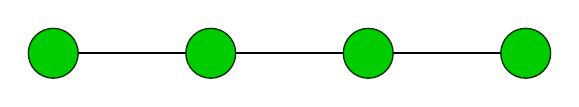
\begin{tikzpicture}
      \SetVertexMath
      \SetVertexNoLabel
      \SetVertexSimple[LineColor=green!20!black,FillColor=green!80!black,MinSize=18pt]
      \grPath[RA=2,RS=5]{4}
      \end{tikzpicture}
    \end{center}
  \item When $n$ is odd, $\nu{(G)}=\lfloor{{n}\over{2}}\rfloor=\tau{(G)}$
    \begin{center}
      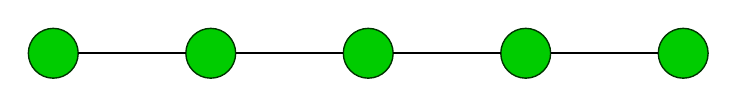
\begin{tikzpicture}
      \SetVertexMath
      \SetVertexNoLabel
      \SetVertexSimple[LineColor=green!20!black,FillColor=green!80!black,MinSize=18pt]
      \grPath[RA=2,RS=5]{5}
      \end{tikzpicture}
    \end{center}
  \end{itemize}
\end{frame}

\begin{frame}
  \frametitle{Observation 2 cont.}
  \begin{exampleblock}{Observation 2}<+->
   Given a connected bipartite graph $G=(V,E)$, if $\nu{(G)}<\tau{(G)}$, then $G$ is not a path nor a cycle.
  \end{exampleblock}
  \begin{itemize}[<+->]
  \item If $G$ is a cycle with $n$ vertices ...
  \item When $n$ is even, then $\nu{(G)}={{n}\over{2}}=\tau{(G)}$
    \begin{center}
      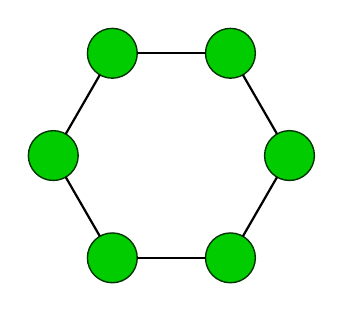
\begin{tikzpicture}
      \SetVertexMath
      \SetVertexNoLabel
      \SetVertexSimple[LineColor=green!20!black,FillColor=green!80!black,MinSize=18pt]
      \grCycle[RA=1.5,RS=5]{6}
      \end{tikzpicture}
    \end{center}
  \end{itemize}
\end{frame}

\begin{frame}
  \frametitle{Observation 2 cont.}
  \begin{exampleblock}{Observation 2}<+->
   Given a connected bipartite graph $G=(V,E)$, if $\nu{(G)}<\tau{(G)}$, then $G$ is not a path nor a cycle.
  \end{exampleblock}
  \begin{itemize}
  \item<+-> What if $n$ is odd?
    \begin{center}
      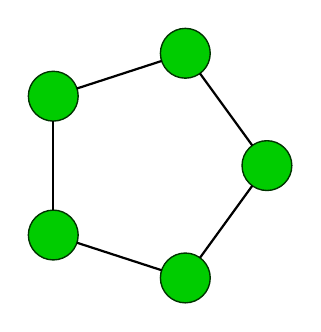
\begin{tikzpicture}
      \SetVertexMath
      \SetVertexNoLabel
      \SetVertexSimple[LineColor=green!20!black,FillColor=green!80!black,MinSize=18pt]
      \grCycle[RA=1.5,RS=5]{5}
      \end{tikzpicture}
    \end{center}
  \item<+-> $\nu{(G)}=2$, but $\tau{(G)}=3$, \uncover<+->{\alert{YOOOOOOOOOOOOOO!}}
  \item<+-> Did we find the new world? \uncover<+->{\alert{NO}}
  \end{itemize}
\end{frame}

\begin{frame}
  \frametitle{Observation 2 cont.}
  \begin{block}{Note}<+->
   If a graph $G$ is an \alert{odd cycle}, then $G$ is \alert{NOT} a bipartite graph.
  \end{block}
  \begin{itemize}[<+->]
  \item It's trivial by using \textsc{Bicolouring Algorithm}
  \item \alert{\textsc{Bicolouring Algorithm}}: decide whether graph $G$ is bicolouring or not in $O(n+m)$ time.
  \end{itemize}
  \begin{exampleblock}{Property}<+->
  If a graph $G$ is bipartite graph iff $G$ is bicolouring.
  \end{exampleblock}
  \begin{alertblock}{Conclusion}<+->
  Thus, $G$ is neither a path nor a cycle, and then it is useful that $G$ exist some vertices whose degree is larger than 3.
  \end{alertblock}
\end{frame}

\begin{frame}
  \frametitle{Idea of Proof}
  \begin{itemize}
  \item<1-> First, prove $\nu{(G)}\leq{\tau{(G)}}$
    \begin{block}{Fact}<3->
    For any graph, $\nu{(G)}\leq{\tau{(G)}}$.
    \end{block}
  \item<2-> Then, show that $\nu{(G)}<\tau{(G)}$ in bipartite graph is impossible.
    \begin{exampleblock}{Observations and Lemma}<4->
    \begin{itemize}
    \item Observation 1 (done): Given a bipartite graph $G=(V,E)$, if $\nu{(G)}<\tau{(G)}$, then there exists a component $G^{'}$ in $G$ where $\nu{(G^{'})}<\tau{(G^{'})}$.
    \item<5-> Observation 2 (done): Given a connected bipartite graph $G=(V,E)$, if $\nu{(G)}<\tau{(G)}$, then $G$ is not a path nor a cycle.
    \item<6-> Lemma (\alert{todo}): Given a connected bipartite graph $G$, $G$ is neither a path nor a cycle, then $\nu{(G)}=\tau{(G)}$.
    \end{itemize}
    \end{exampleblock}
  \end{itemize}
\end{frame}

\begin{frame}
  \frametitle{Idea of Proof (cont.)}
  \begin{exampleblock}{K\"{o}nig's Matching Theorem}<+->
    If a graph $G=(V,E)$ is a bipartite graph, then $\nu{(G)}=\tau{(G)}$
  \end{exampleblock}
  \begin{itemize}[<+->]
  \item Proof:
  \item By the Fact, we know that $\nu{(G)}\leq{\tau{(G)}}$ for all graph $G$
  \item By Observation 1 \& 2 and Lemma, we prove the theorem.
  \end{itemize}
\end{frame}

\begin{frame}
  \frametitle{Lemma}
  \begin{exampleblock}{Lemma}<1->
  Given a connected bipartite graph $G$, $G$ is neither a path nor a cycle, then $\nu{(G)}=\tau{(G)}$.
  \end{exampleblock}
  \begin{alertblock}{Technique}<2->
  Suppose a minimal counterexample $G$, i.e. for all subgraph $H$ of $G$ hold $\nu{(H)}=\tau{(H)}$ except $G$ which holds $\nu{(G)}<\tau{(G)}$.
  \end{alertblock}
  \begin{itemize}
  \item<3-> Let $u$ be the vertex where $\deg{(u)}\geq{3}$, $e=(u,v)\in{E(G)}$, and $H=G\setminus{\{v\}}$
  \item<4-> I think there are 2 cases when first reading the paper:
    \begin{enumerate}
    \item<5-> $\nu{(H)}<\nu{(G)}$ \uncover<7->{$\Rightarrow$ $e\in{M_G}$ (Haha I'm smart)}
    \item<6-> $e\notin{M_G}$
    \end{enumerate}
  \end{itemize}
\end{frame}

\begin{frame}
  \frametitle{Lemma cont.}
  \begin{itemize}
  \item<1-> But ...
    \begin{enumerate}
    \item<2-> $e\in{M_G}$ \uncover<8->{\alert{DO NOT} forget $\nu{(H)}<\nu{(G)}$}
      \begin{itemize}
      \item<3-> $u\in{W_G}$ \uncover<6->{... maybe $\tau{(H)}=\tau{(G)}$ or $\tau{(H)}<\tau{(G)}$}
      \item<3-> $v\in{W_G}$ \uncover<6->{... maybe $\tau{(H)}=\tau{(G)}$ or $\tau{(H)}<\tau{(G)}$}
      \end{itemize}
    \item<2-> $e\notin{M_G}$ \uncover<8->{\alert{DO NOT} forget $\nu{(H)}=\nu{(G)}$ or $\nu{(H)}<\nu{(G)}$}
      \begin{itemize}
      \item<4-> $u\in{W_G}$ \uncover<7->{... maybe $\tau{(H)}=\tau{(G)}$ or $\tau{(H)}<\tau{(G)}$}
      \item<4-> $v\in{W_G}$ \uncover<7->{... maybe $\tau{(H)}=\tau{(G)}$ or $\tau{(H)}<\tau{(G)}$}
      \item<5-> Note that both $u,v\notin{W_G}$ is impossible 
      \end{itemize}
    \end{enumerate}
  \item<9-> Actually, there are \alert{many} cases. (Haha UCCU)
  \end{itemize}
  \uncover<10->{\begin{center}
    \includegraphics[width=6cm]{foo.png}
  \end{center}}
\end{frame}

\begin{frame}
  \frametitle{Lemma cont.}
  \begin{enumerate}[<+->]
  \item If $\nu{(H)}<\nu{(G)}$
    \begin{itemize}
    \item exists $W_H$ where $|W_H|=\tau{(H)}=\nu{(H)}<\nu{(G)}$
    \item $W_H\cup{\{v\}}$ is a cover of $G$, $|W_H\cup{\{v\}}|=\tau{(G)}$
    \item thus, $\tau{(G)}=|W_H\cup{\{v\}}|=\tau{(H)}+1=\nu{(H)}+1\leq{\nu{(G)}}$
      \begin{block}{Fact}
      For any graph, $\nu{(G)}\leq{\tau{(G)}}$.
      \end{block}
    \item $\Rightarrow$ $\nu{(G)}=\tau{(G)}$, a contradiction!
    \end{itemize}
  \item If $\nu{(H)}=\nu{(G)}$
    \begin{exampleblock}{Note}
    If $\nu{(H)}=\nu{(G)}$, then $e\notin{M_G}$.
    \end{exampleblock}
  \end{enumerate}
\end{frame}

\begin{frame}
  \frametitle{Lemma cont.}
  \begin{exampleblock}{Note}<+->
  If $\nu{(H)}=\nu{(G)}$, then $e\notin{M_G}$.
  \end{exampleblock}
  \begin{itemize}[<+->]
  \item Assume $v$ is \alert{NOT} incident with any of edge in $M_G$
  \item Then, exist an edge $f=(u,v^{'})\in{E(G\setminus{M_G})}$, and $v\neq{v^{'}}$ \uncover<+->{\alert{$\deg{(u)}\geq{3}$}}
  \item Let $G^{'}=G\setminus{\{f\}}$, we can find a minimum cover $W_{G^{'}}$ with $|W_{G^{'}}|=\tau{(G^{'})}=\nu{(G^{'})}=\nu{(G)}$
  \item Since $v$ is not incident with any of edge in $M_G$ $\Rightarrow$ $v\notin{W_{G^{'}}}$
  \item $\Rightarrow$ $u\in{W_{G^{'}}}$ and thus $W_{G^{'}}$ be a cover of $G$
  \item $\Rightarrow$ $\nu{(G)}=|W(G^{'})|\geq{\tau{(G)}}$
  \item $\nu{(G)}=\tau{(G)}$
  \end{itemize}
\end{frame}

\end{document}